% !TEX root = ../The-Haptic-Printer.tex
%
\chapter{Architecture}
\label{sec:architecture}

\cleanchapterquote{Any application that can be written in JavaScript, will eventually be written in Javascript.}{Jeff Atwood}{Code Horror (blog)} 

This section describes the usage and mapping of hardware and software of this application. This section 
will clear out some questions about the application like. How the application
is consuming the inputs? How the application is transforming the data states to finally in the output? 
How are the middle layers processing the data? including some other questions about communication of different components.
The aim of this section is to explain in detail the architecture of the application and flow of features. This will also 
explain the requirements to execute the application on local system.

\begin{figure}[htb]
	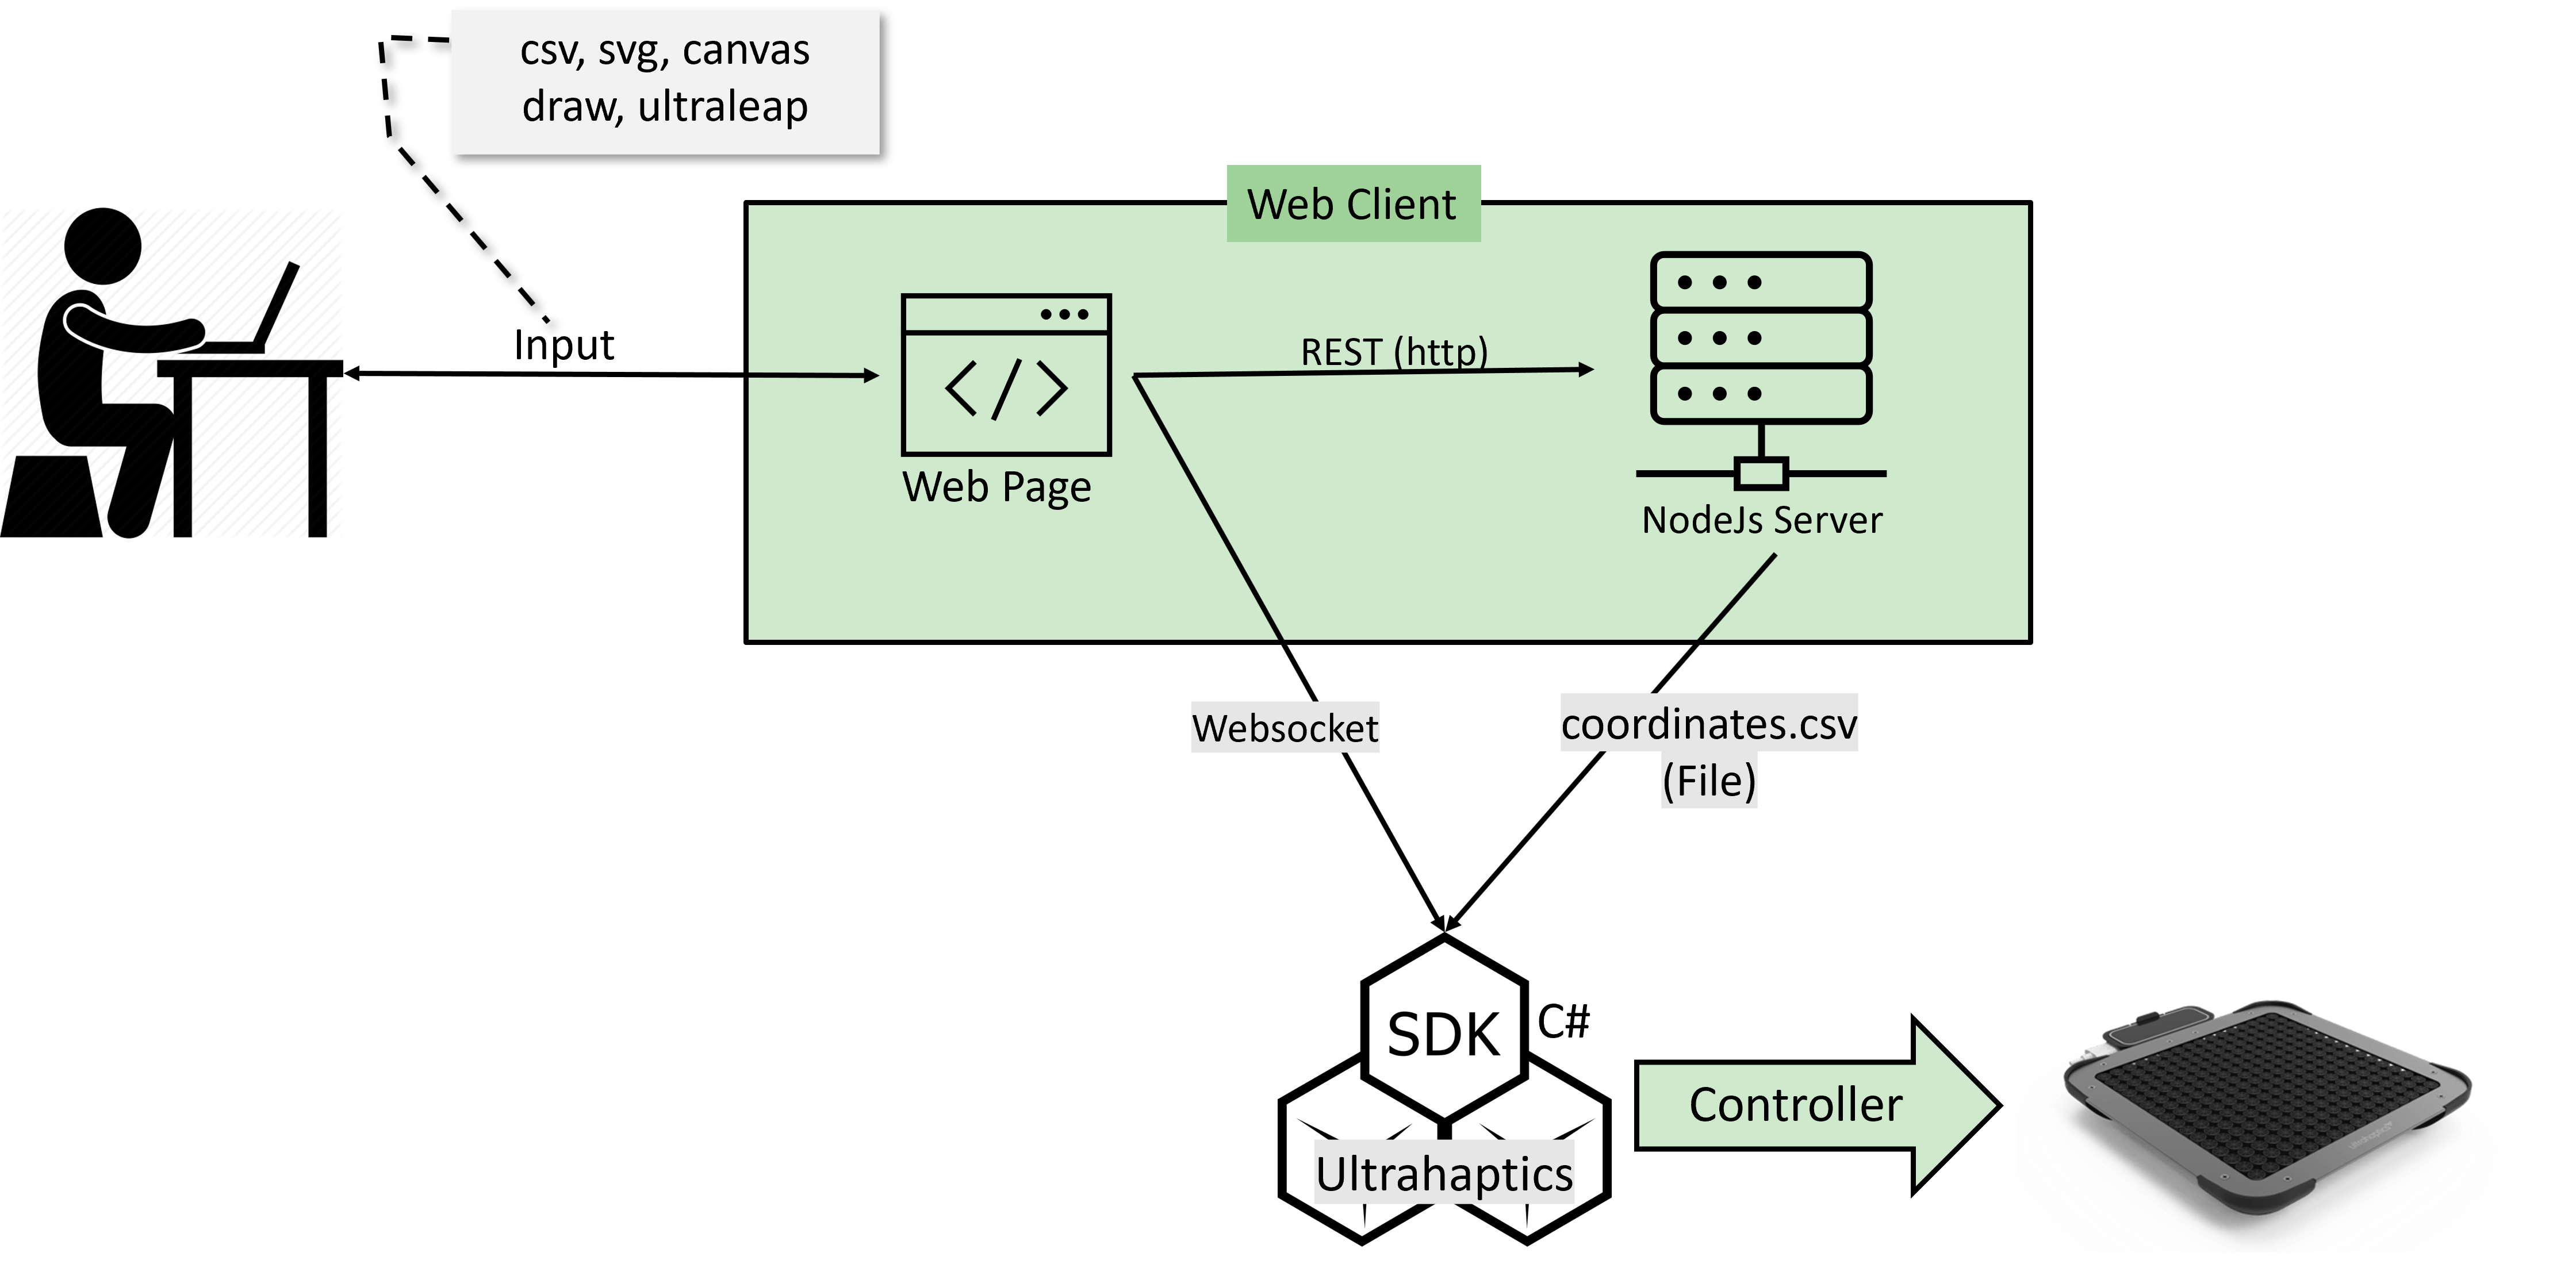
\includegraphics[width=\textwidth]{gfx/Ultrahaptics-custom-architecture}
	\caption{Figure: The Haptic Printer (Application architecture)}
	\label{fig:architecture:overall architecture}
\end{figure}


As seen in the architectural diagram(Fig 4.1) there are multiple components of
 the application, from user 
input to ultrahaptics device to the communication through websocket and REST. 
The components are mentioned in detail below:\\

\section{Frontend}
The front end of the application is the web. The web application is built in 
vanilla-JS served over a nodeJs Server. However, for compiling 
js code for browser babeljs\cite{babel7.15} is used.

\subsection*{The WebApp and Inputs}
The webpage is responsible for taking multiple inputs from the user and start and stop Ultrahaptics device.
The inputs are in form of the canvas draw, SVG icons, CSV file with (x, y) coordinates, Ultraleap inputs. 
The web page is responsible to scale and center the coordinates (according to x/y plane) taken from multiple input types to the 
Ultrahaptics dimensions and units.\\
In case of SVG some more processing is required. Since, there is no direct feature provided by the 
browser to extract the coordinates from an SVG. The code written for this is a custom implementation inspired from a 
spotify tool\cite{spotify-coordinator} which is under Apache license 2.0 . After extracting the coordinates from the 
given input the coordinates are scaled according to the output device and sent to the backend server in NodeJs, 
the processing in the nodeJs is explained in the section backend. \\
After, the successful response from the Node Server the front end is also responsible to communicate to the 
Ultrahaptics SDK implementation to start and stop the Ultrahaptics rendering.

\section{Backend}

The Backend is further divided into two parts. The First, is the Node Js Server. Second is, the system implementation 
in C-sharp, which is responsible to control and render shapes in Ultrahaptics device. \\[4mm]
\subsection*{NodeJs Server} 
The functionality of nodeJS server is minimal. It hosts the WebApp at localhost:3000 in its root and also 
consumes the scaled coordinates from the WebApp. After getting the coordinates it creates a CSV file and writes 
all the coordinates in a csv as x,y as two columns. Post this functionality it responds to the webapp with a success message. 
This CSV file is later consumed by the SDK API implementation to render it on Ultrahaptics device.\\[4mm]

\subsection*{The SDK extension: Ultrahaptics API's} 
Ultrahaptics SDK\cite{Ultrahaptics-APIs} has provided some of the classes to manipulate the control points, 
intensity and how the emitter will respond to the control points and positions provided to it. We built a 
system using these API's to continuously render custom points and shapes provided. 
All the previous implementations and tests we found were for a shapes which were pre defined in the code 
and it was a challenge to dynamically change the emitter points at a given time.  \\
This part of the system implements two types of rendering Amplitude Modulation(AM) and Time Point Streaming(TPS).
Both the implementations consumes dynamic inputs and detail explanation of how it is implemented 
can bee seen below in code documentation in Files AM.cs and TPS.cs. The choice of rendering type 
between AM and TPS can be selected from the WebApp. \\
The system also implements a websocket for communication which will be discussed further. 

\section{Communication}
\subsection*{Websocket}
The websocket communication happens between the web app and Csharp Ultrahaptics system to consume API's.
Where Csharp implements the websocket server $(for reference, see file UltrahapticsOrchestrator.cs)$ and webapp implements the 
websocket client $(ref see cswebsocket.js below)$. The webapp sends a message to backend system to start or stop the
Ultrahaptics device rendering, using websocket. It also sends what type of rendering to use(AM or TPS). the websocket 
communication message is in JSON format and an example message can be seen below.
\begin{figure}[htb]
	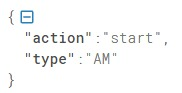
\includegraphics[width=40mm]{gfx/jsonstart.jpeg}
	\caption{Figure: Json example to start AM rendering}
	\label{fig:architecture:json}
\end{figure}

\subsection*{REST}
The REST communication in between the webapp and the NodeJs server. After the input processing in the webapp the coordinates are sent to 
the NodeJs usin this REST channel at $localhost:3000$.  
\subsection*{CSV file I/O}
After the NodeJs server receives the coordinates, the coordinates are written to a csv file in the column format. 
Column names (x,y). These coordinates file is picked up 

